\chapter{Algoritmi per le impronte digitali}

\section{Algoritmi di prefiltraggio ed enhancement}

Nel modulo per \textbf{estrazione delle feature} si eseguono
tipicamente questi passi:
\begin{enumerate}
    \item filtraggio iniziale
    \item manipolazione dell'immagine (enhancement)
    \item estrazione delle feature
    \item codifica
\end{enumerate}

\begin{figure}[ht]
    \centering
    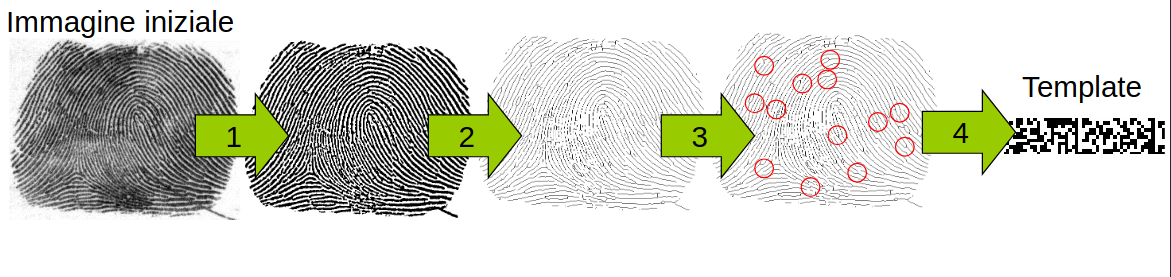
\includegraphics[width=1\linewidth]{chapters/images-chap6/estrazione-fet.png}
\end{figure}

In questa sezione ci concentriamo sui punti 1 e 2.

\subsection{Filtraggi iniziali}

\subsubsection{Contrast streching}
Le immagini delle impronte digitali hanno di
solito una dinamica dei toni di grigio molto
limitata; l’operazione di Contrast Stretching allarga la
dinamica dell’immagine.

\begin{figure}[ht]
    \centering
    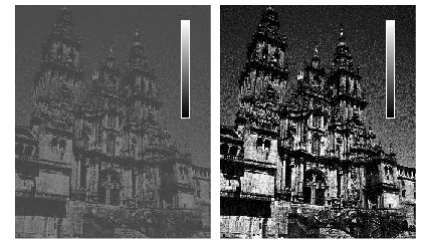
\includegraphics[width=0.5\linewidth]{chapters/images-chap6/constrast-stre.png}
\end{figure}

\subsubsection{Manipolazione dell'istogramma}

L’istogramma di una
immagine può essere
mappato in un altro
mediante diverse
funzioni; il logaritmo permette
ad esempio di
evidenziare delle
variazioni sottili di toni
di grigio in una
immagine che ha già
una dinamica elevata.

\begin{figure}[ht]
    \centering
    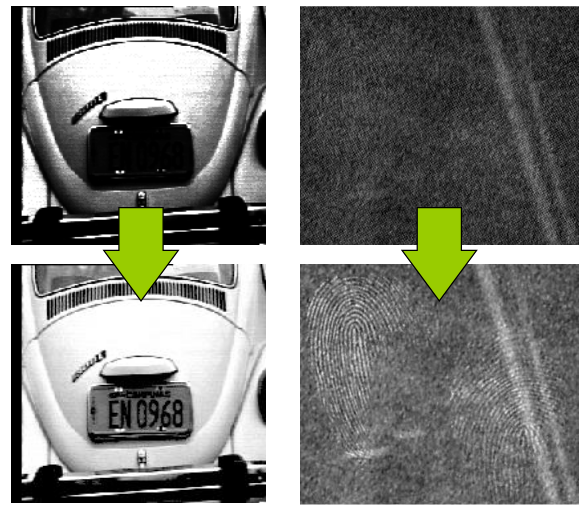
\includegraphics[width=0.5\linewidth]{chapters/images-chap6/man-isto.png}
\end{figure}

\subsubsection{Filtro di Wiener}

Quando si conoscono le caratteristiche spettrali
dell’immagine e del rumore si usa il filtro di
Wiener. Si riesce a distinguire i rumori tra sfondo ed impronta, dando risalto al secondo.

\begin{figure}[ht]
    \centering
    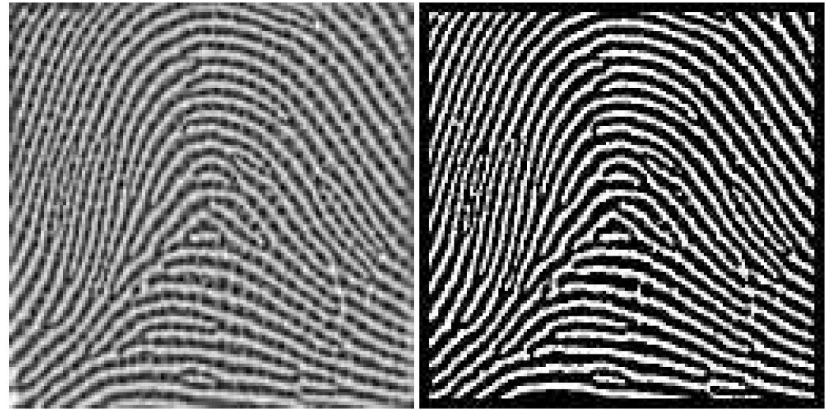
\includegraphics[width=0.5\linewidth]{chapters/images-chap6/filtro-we.png}
\end{figure}

\subsubsection{Normalizzazione}

L’obiettivo della normalizzazione è quello di standardizzare le
variazione di grigio dei ridge in tutta l’immagine per agevolare
gli algoritmi successivi.

\subsubsection{Segmentazione}

Gli algoritmi per la segmentazione estraggono il foreground
dal background (impronta dallo sfondo).

Permettono di focalizzarsi solo sulle regioni della immagine che 
portano informazione utile al processo biometrico.

\subsubsection{Regioni con diversa qualità}

Una volta che l’impronta è stata individuata nella immagine
dalla segmentazione si iniziano le analisi successive.

Una volta che l’impronta è stata individuata nella immagine
dalla segmentazione si iniziano le analisi successive:
\begin{itemize}
    \item diversa pressione
    \item traslazioni
    \item tagli
    \item uso non corretto dell'inchiostro
\end{itemize}

Di solito si distinguono tre regioni:
\begin{itemize}
    \item well-defined
    \item recoverable
    \item unrecovable
\end{itemize}

\subsection{Manipolazione dell'immagine}

Ha due obiettivi:
\begin{itemize}
    \item \textbf{migliorare la chiarezza della struttura dei ridge} dove possibile
    \item \textbf{marcare le regioni dove non è possibile estrarre informazione} perché c'è troppo rumore
\end{itemize}

Prende in ingresso una immagine di toni di grigio, e produce un'immagine 
a toni di grigio binarizzata.

\subsubsection{Filtri contestuali}

Per ottenere i massimi risultati nell‘evidenziare la
struttura dei ridge in una immagine occorre ricorrere ai
filtri adattativi o contestuali. Questa categoria dei filtraggi per le immagini modifica
automaticamente i propri parametri per meglio adattarsi
al mutare delle condizioni dell’immagine, basandosi su:
\begin{itemize}
    \item distanza tra i ridge
    \item orientamento dei ridge
    \item livello di rumore presente
\end{itemize}

Questi filtri lavorano sulla immagine in ingresso
attraverso un’operazione chiamata convoluzione con una
maschera di filtraggio.

A seconda del tipo di maschera usata il filtro
aumenta/diminuisce alcune caratteristiche piuttosto che
altre.

\subsubsection{Filtro di O'Gorman e Nickerson}

La forma particolare di questa maschera è fatta per fare
“match” con lo spessore dei ridge, la loro distanza di
separazione, il valore del massimo e del minimo in un
intorno del punto di esame.

Questo filtro tende ad attenuare il rumore locale.

\section{Estrazione di caratteristiche}

Ci concetriamo sull'estrazione delle feature di I livello (direzione dei ridge, core, delta, ridge count).

\subsection{Ridge counting}

E’ una misura dei ridge che attraversano una
linea immaginaria passante tra due minutiae.

\begin{figure}[ht]
    \centering
    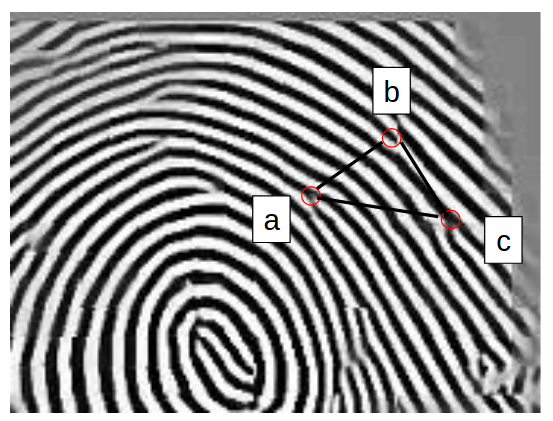
\includegraphics[width=0.5\linewidth]{chapters/images-chap6/ridge-counting.png}
\end{figure}

\begin{itemize}
    \item fra A e B 4 ridge
    \item fra B e C 0 ridge
    \item fra C e A 3 ridge
\end{itemize}

\subsection{Analisi delle frequenze spaziali}

E’ una misura di quanto sono stretti o larghi i
ridge nelle varie regioni dell’impronta.

\begin{figure}[ht]
    \centering
    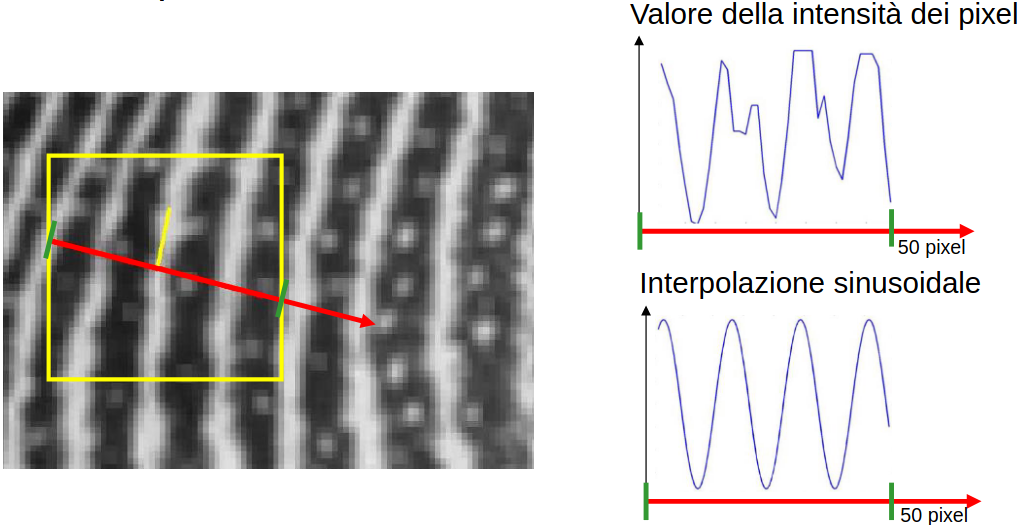
\includegraphics[width=1\linewidth]{chapters/images-chap6/ridge-freq.png}
\end{figure}

\subsubsection{Mappa delle frequenze spaziali}

Usando l’informazione ricavata dalle frequenze di
ridge per ogni blocco dell’immagine è possibile
avere la mappa delle frequenze dell’immagine.



